% Use the temporary template.
\documentclass{aiaa-pretty}

% Author information
\author[Hastings, Dohnson, and Brooks]{ %
Nedward N. Hastings\thanks{Graduate Research Assistant, Department of Aerospace Engineering, AIAA Student Member, \texttt{hastings@bysu.edu}},
Darcie J. Dohnson\thanks{Graduate Research Assistant, Department of Aerospace Engineering, AIAA Student Member, \texttt{dohnson@bysu.edu}},
Geromie R. Brooks\thanks{Professor, Department of Aerospace Engineering, AIAA Fellow, \texttt{brooks@bysu.edu}}\\
\textit{Bowling Yellow State University, Springfield, MD 69743}}

% Title
\title{An Improved Algorithm for Solving Equations of One Variable}

% Abstract
 \abstract{ %
  This paper demonstrates the use of a particular template.  In the mean time, it discusses algorithms to solve nonlinear equations of a single variable.  This is a subject that lends itself well to simple equations and the use of a few figures and tables.  This should be enough to demonstrate the main features of this package using a small number of pages.}


% Begin the document
\begin{document}
% Insert the title.
\maketitle

\section{Introduction}
There is a need in almost all scientific disciplines\footnote{And many disciplines that are not scientific} to be able to solve equations of the form
\begin{equation}
f(x)=0
\end{equation}
where the function $f:\mathbb{R}\to\mathbb{R}$ cannot be inverted symbolically.  This can occur with even relatively simple equations, for example
\begin{equation}
f(x)=x - \sinh x
\end{equation}
Many texts, for example \cite{chapra:2002:numerics}, have chapters on this subject.  A common technique to address such problems is to use an iterative algorithm, in which the values of the function at previous estimates are used to obtain the new estimates of the value of $x$ that satisfy the equation.  Consider as an example Newton's method, which is one of the most common techniques.
\begin{equation}
x_{n+1} = x_n - \frac{f(x_n)}{f'(x_n)}
\end{equation}
In this case, the value of the function and its derivative at only the previous iteration is used to determine the next estimate.  Ideally, $f(x_n)\to 0$ as $n\to\infty$ (and this is often in fact the case).

Methods like Newton's method that only use one previous estimate at a time can have very good performance, but they are also prone to failure \cite{ypma:1995:newton-raphson}.  As a simple example, consider
\begin{equation}
f(x) = \tanh x
\end{equation}
Provided the initial estimate, $x_0$ is a real number other than zero, applying Newton's method gives the result
\begin{equation}
\lvert x_{n+1} \rvert > \lvert x_n \rvert
\end{equation}
despite the fact that the solution is at $x=0$.  A more robust class of methods can be used when we have two real numbers $a<b$ such that
\begin{equation}
f(a)f(b) < 0
\end{equation}
Provided that $f$ is a continuous function, the intermediate value theorem, \cite{rudin:1976:analysis}, guarantees that there is some $a < x < b$ such that $f(x)=0$.  If we also assume that $f$ is strictly monotonic, then this value of $x$ is unique.

When we have $f$, $a_n$, and $b_n$ that satisfy these criteria, we can select some value $s_n \in (a_n,b_n)$ and evaluate it.  If $f(a_n)f(s_n)<0$, we know that the solution is between $a_n$ and $s_n$, and we update using
\begin{align}
a_{n+1}&=a_n & b_{n+1}&=s_n
\end{align}
If $f(a_n)f(s_n)>0$, we update using
\begin{align}
a_{n+1}&=s_n & b_{n+1}&=b_n
\end{align}
Of course, if $f(s_n)=0$, we terminate the algorithm because $s_n$ is an exact solution.  Any algorithm that follows this outline is called a bracketing method, which is the main subject of this paper.

\section{Numerical Techniques}  \label{sec:techniques}
Two functions that satisfy the assumptions for a bracketing method are shown in Fig.~\ref{fig:f:plain}.  The example in Fig.~\ref{fig:f:2} is particularly difficult to solve because the function has very little gradient information away from the root.

\begin{figure}
 \centering
 \subfigure[\label{fig:f:1}Type 1 challenge] %
  {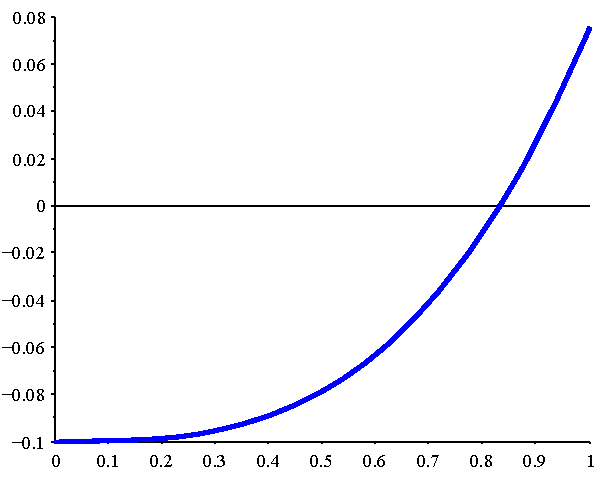
\includegraphics[width=3.05in]{./pics/f1_plain.pdf}}
 \subfigure[\label{fig:f:2}Type 2 challenge] %
  {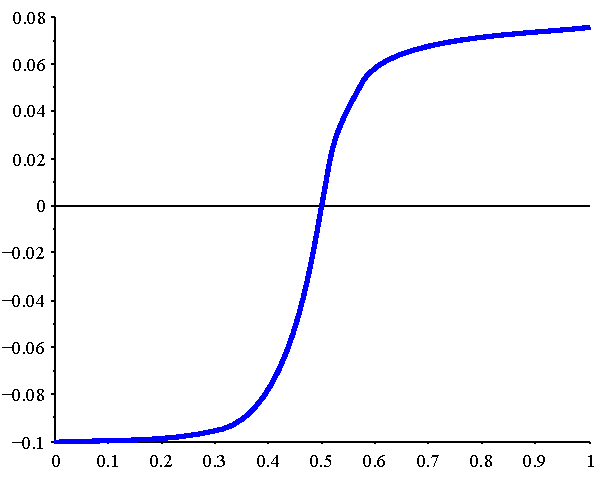
\includegraphics[width=3.05in]{./pics/f2_plain.pdf}}
 \caption{ \label{fig:f:plain}
  Two examples of functions that satisfy the bracketing assumptions}
\end{figure}


\subsection{Convergence Criteria} \label{ssec:criteria}
Figure \ref{fig:f:tol} gives a visualization for the uncertainty in both axes for several iterations of a bracketing scheme.  The yellow circles represent the iterative upper and lower bounds for the root location, and the sequentially darker orange boxes represent the current estimate of the region in which the root must exist.  Of course, we know that the root must lie on the $x$-axis, but the height of the box still gives a good representation of how good the current estimate is.  \href{http://www.google.com}{Google}

\begin{figure}
 \centering
 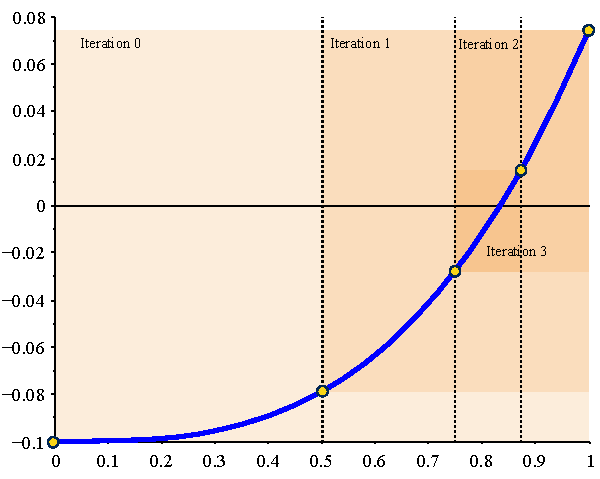
\includegraphics[width=3in]{./pics/f1_tol.pdf}
 \caption{ \label{fig:f:tol}
  Residuals in $x$- and $y$-directions}
\end{figure}


\subsection{Methodology}



\section{Results}
Here is a reference to Section \ref{sec:techniques}.\ref{ssec:criteria}.


\section{Conclusions}                            \label{sec:conclusion}
A reduced-order two-dimensional model was developed that can analyze shock waves, expansion fans, and finite-rate chemistry.  The model was found to be particularly accurate in determining the boundary of the exhaust plume, which is essential to thrust calculations.  Recombination can also be modeled as long as the flow is well-mixed before reaching the nozzle.  However, the importance of recombination to thrust calculations was debatable, even for a set of conditions specifically selected to emphasize the importance of recombination.

The model does not have the capability to analyze boundary layers, which were found to play an important role.  The boundary layer had a noticeable effect on all quantities except for pressure.  These results make a strong case that a boundary layer model must be added to the reduced-order model.

\begin{figure}[!h]
 \begin{center}
  Whatever
 \end{center}
 \caption{Test figure}
\end{figure}

\aiaaappendix{Brent's Method}

\appendix
\section{Another Thing}


\section*{Acknowledgements}
This document was prepared by Derek Dalle with help from Sara Spangelo.  The names, universities, towns, and email addresses are not intended to refer to real people, places, or objects.

% References
\bibliographystyle{aiaa}
\bibliography{./bib/aiaa-sample}


\end{document}
